\documentclass[10pt, aspectratio=169]{beamer}
\usetheme{metropolis}

\usepackage[T2A]{fontenc}
\usepackage[utf8]{inputenc}
\usepackage[russian]{babel}
\usepackage{graphicx}
\usepackage{hyperref}
\usepackage{amsmath}
\usepackage{listings}
\usepackage{xcolor}
\usepackage{qrcode}

\title{Современная экосистема университетской навигации}
\subtitle{Панорамные карты, маршрутизация и интегрированные коммуникации}
\institute{Челябинский государственный университет}
\date{\today}

\begin{document}

\begin{frame}[plain]
	\titlepage
\end{frame}


\begin{frame}{Обоснование проекта}
	\begin{itemize}
		\item Замена для \href{https://map.csu.ru}{map.csu.ru}
		\item Потребность в современной панорамной съемке 360°
		\item Отказ от старой кодовой базы по причинам:
		      \begin{itemize}
			      \item Низкая экономическая эффективность (технический долг)
			      \item Необходимость в современном стеке технологий
		      \end{itemize}
	\end{itemize}
\end{frame}

\begin{frame}{Цели проекта}
	\begin{itemize}
		\item Интерактивный редактор карт с 3D-изображениями
		\item Интеграция событий и расписания, поиск кратчайших маршрутов
		\item Внутренние коммуникации: сервер ejabberd + веб-клиент
		\item Инструменты импорта данных (парсеры) или ручной ввод расписания
	\end{itemize}
\end{frame}


\begin{frame}{Текущие проблемы}
	\begin{itemize}
		\item Отсутствие единой защищенной среды для общения в реальном времени
		\item Децентрализация информационных ресурсов университета
		\item Низкая эффективность каналов оповещения
	\end{itemize}
	\vfill
	\textbf{Решение:} агрегация сервисов в едином интерфейсе.
\end{frame}

\begin{frame}{Основные принципы разработки}
	\begin{itemize}
		\item Безопасность, производительность, портативность, поддерживаемость
		\item Соответствующий выбор стека технологий
		\item Исключены: Python (неполностью), JavaScript, C\# (несоответствие по производительности / архитектуре)
		\item Цель: получение опыта работы с high-load системами, решение текущих проблем.
	\end{itemize}
\end{frame}

\begin{frame}{Визуализация панорамного контента}
	\begin{itemize}
		\item Эквидистантная проекция для изображений 360°
		\item Реализация с помощью \texttt{three.js} (виртуальная сфера / кубический маппинг)
		\item Сегментированная загрузка (тайлинг) для изображений 8K+
	\end{itemize}
\end{frame}

\begin{frame}{Основы маршрутизации}
	\begin{itemize}
		\item Взвешенный ориентированный граф (двойственность Пуанкаре)
		\item Вершинами являются аудитории и двери, а ребрами~--- узлы связи между точками интереса.
		\item IndoorGML + \texttt{pgRouting} для динамической фильтрации подграфов
		\item Кратчайший путь по алгоритму Дейкстры
	\end{itemize}
\end{frame}

\begin{frame}{Протоколы распределенных коммуникаций}
	\begin{itemize}
		\item XMPP --- открытый, расширяемый, на базе XML
		\item Сервер \texttt{ejabberd} --- отказоустойчивость, высокая конкурентность
		\item Возможности:
		      \begin{itemize}
			      \item Обмен сообщениями в реальном времени
			      \item Многопользовательские конференции
			      \item Уведомления
			      \item Изоляция от персональных социальных сетей
		      \end{itemize}
	\end{itemize}
\end{frame}

\begin{frame}{Информационная безопасность}
	\begin{itemize}
		\item \textbf{Shift Left Security} --- раннее обнаружение уязвимостей
		\item Язык Go --- GC, низкая зависимость от рантайма.
		\item Меры защиты:
		      \begin{itemize}
			      \item ORM (предотвращение SQL-инъекций)
			      \item Anubis (защита от ботов)
			      \item Авторизация через JWT
			      \item Middleware, distroless-контейнеры
			      \item Статические анализаторы + Quality Gates в CI/CD
		      \end{itemize}
	\end{itemize}
\end{frame}



\begin{frame}{QR-код --- Обзор архитектуры}
	\centering
	\qrcode[height=5cm]{https://github.com/ylnt241/eng-project/blob/main/images/Overview.drawio.png?raw=true}

	\vspace{1em}

	\text{\href{https://github.com/ylnt241/eng-project}{https://github.com/ylnt241/eng-project}}

	\small{Отсканируйте, чтобы просмотреть схему архитектуры в высоком разрешении}
\end{frame}

\begin{frame}{Общий обзор архитектуры}
	\begin{figure}
		\centering
		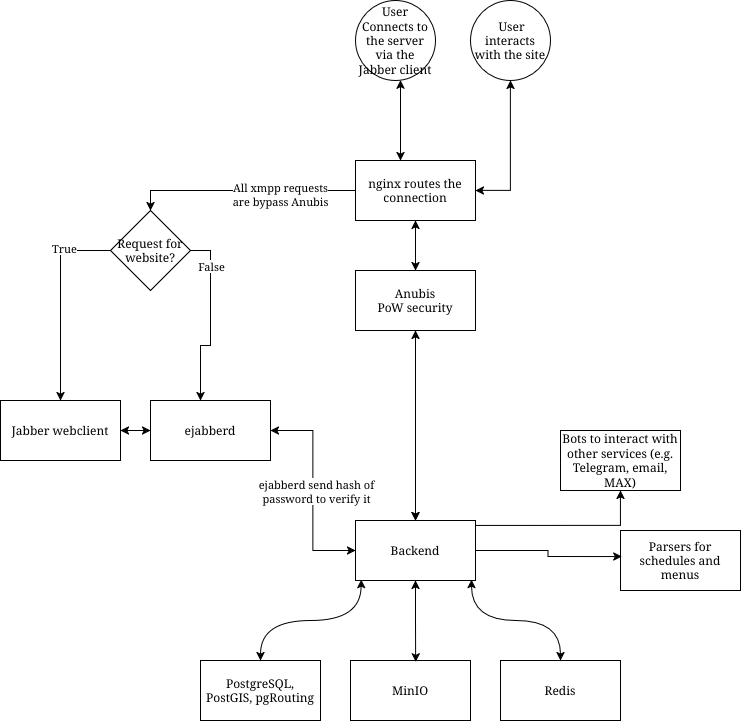
\includegraphics[width=0.7\textwidth, height=0.8\textheight, keepaspectratio]{images/Overview.drawio.png}
		\label{fig:overview}
	\end{figure}
\end{frame}

\begin{frame}{Архитектурные принципы}
	\begin{itemize}
		\item \textbf{Консолидация сервисов:} минимизация количества контейнеров
		\item \textbf{Гибридный монолит:} основная логика в едином бэкенд-сервисе
		\item \textbf{Stateless-подход:} задел для переезда в кубер (ага, щазз)
	\end{itemize}
\end{frame}

\begin{frame}{Технологический стек --- Основные компоненты}
	\begin{itemize}
		\item \textbf{Сеть:} NGINX + Anubis (защита от ботов)
		\item \textbf{Хранение данных:} PostgreSQL + PostGIS + pgRouting
		\item \textbf{Коммуникации:} Ejabberd + XMPP клиент
		\item \textbf{Хранилище объектов и кэширование:} MinIO (S3-совместимое), Redis
		\item \textbf{Внешние сервисы:} парсеры на Python, боты на Go/Python
	\end{itemize}
\end{frame}


\begin{frame}{QR-код --- Структура бэкенда}
	\centering
	\qrcode[height=5cm]{https://github.com/ylnt241/eng-project/blob/main/images/Backend.png?raw=true}

	\vspace{1em}

	\text{\href{https://github.com/ylnt241/eng-project}{https://github.com/ylnt241/eng-project}}

	\small{Отсканируйте, чтобы просмотреть блок-схему бэкенда в высоком разрешении}
\end{frame}

\begin{frame}{Структура бэкенда}
	\begin{figure}
		\centering
		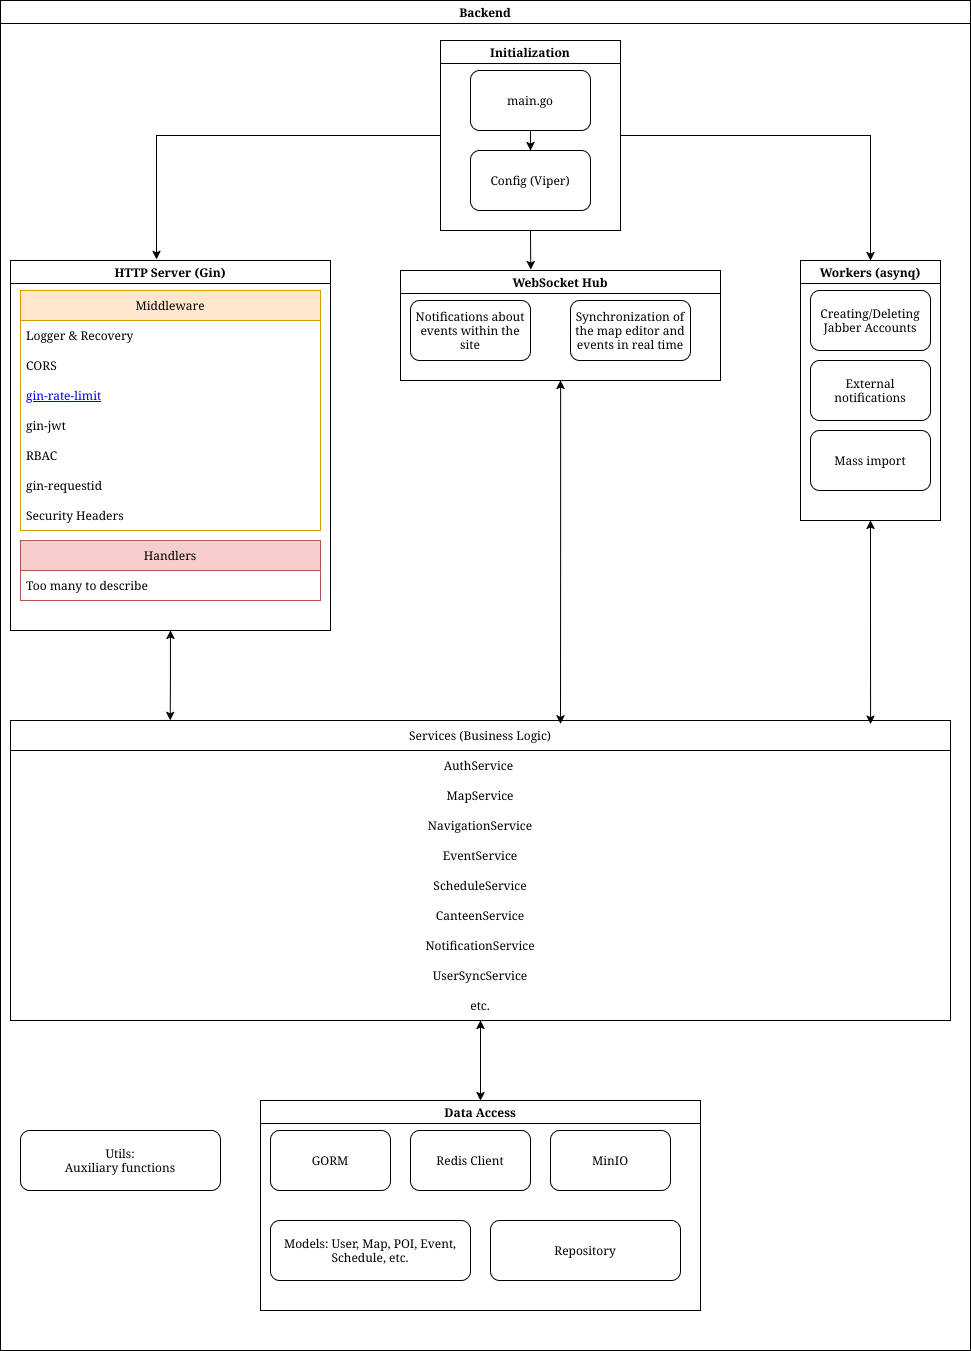
\includegraphics[width=0.7\textwidth, height=\textheight, keepaspectratio]{images/Backend.png}
		\label{fig:backend}
	\end{figure}
\end{frame}

\begin{frame}{Реализация бэкенда (Go)}
	\begin{itemize}
		\item Многослойная архитектура
		\item \textbf{Инициализация:}
		      \begin{itemize}
			      \item Viper для конфигурации
			      \item Автоматические миграции (golang-migrate)
			      \item Клиенты Redis и Asynq
			      \item DI
		      \end{itemize}
		\item \textbf{Транспорт:} фреймворк Gin, WebSocket-хаб
	\end{itemize}
\end{frame}

\begin{frame}{DevOps и безопасность}
	\begin{itemize}
		\item \textbf{CI/CD через Jenkins:}
		      \begin{itemize}
			      \item Автоматические тесты для каждого PR
			      \item Статический анализ SonarQube + Quality Gates
			      \item Обязательное код-ревью
		      \end{itemize}
		\item \textbf{Контейнеризация:}
		      \begin{itemize}
			      \item Образы Distroless --- минимальная поверхность атаки
			      \item Многоэтапные сборки (Multi-stage builds)
			      \item Анализ контейнеров
		      \end{itemize}
	\end{itemize}
\end{frame}

\begin{frame}{Мониторинг и защита}
	\begin{itemize}
		\item Фильтрация через Middleware (SQL-инъекции, XSS)
		\item Anubis + NGINX --- блокировка вредоносного трафика
		\item Обеспечение доступности в условиях ограниченных ресурсов
		\item Хочется WAF, но мы, объективно, не тянем по ресурсам.
	\end{itemize}
\end{frame}

\section*{Заключение}

\begin{frame}{Заключение}
	\begin{itemize}
		\item Современная навигационная экосистема с панорамами 360°
		\item \textbf{Ключевые цели:}
		      \begin{itemize}
			      \item Высокопроизводительный бэкенд на Go
			      \item pgRouting + графовая модель для внутренней навигации
			      \item Shift Left Security, distroless-контейнеры
			      \item Stateless, масштабируемая архитектура
		      \end{itemize}
		\item Улучшение цифрового взаимодействия для студентов и сотрудников
	\end{itemize}
\end{frame}

\begin{frame}{Конец.}
	\centering
	\vfill
	\Large{Спасибо за внимание.}
	\vfill
\end{frame}

\end{document}
